{\color{secblue}\subsection{Other design decisions}}
{\color{secblue}\subsubsection{ER schema}}
The following is the ER schema of the database. It shows how the users' data is organized for the authentication, the Data4Help service and the Track4Run service. Obviously the AutomatedSOS service doesn't appear because there is no data that need to be stored for a user.
\begin{figure}[H]
    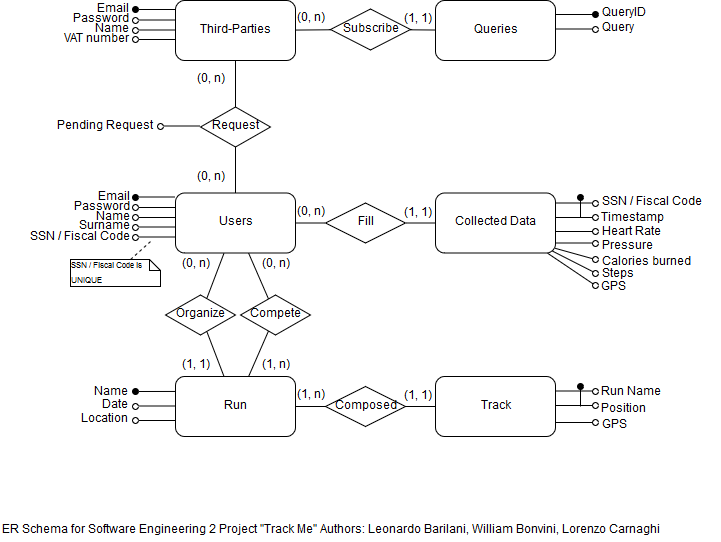
\includegraphics[width=\linewidth, keepaspectratio]{./Images/er.png}
    \centering
    \caption{ER Diagram}
    \label{fig:depview}
  \end{figure}
{\color{secblue}\subsubsection{AutomatedSOS optimization}}
Regarding the AutomatedSOS service there are two optimizations:
\begin{itemize}
\item The first optimization consists in memorizing the list of the available hospitals in the configuration files of the Automated SOS Forwarder component and not in the AWS instance. This way when an emergency occurs the component has already all the information that he needs and doesn't have to make queries that can slow down the entire process;
\item The second optimization aims at lightening the amount of packets from the user to the server: tipically every packet that a user sends is marked with the services that the user is subscribed to, no matter what happens. With AutomatedSOS this is not true: a packet is marked as an AutomatedSOS packet only if the Automated SOS app detects an emergency. If the user uses only the Automated SOS' app than a packet is sent only if there is an emergency. This way we cut useless packets traffic and we lighten the load on the server.
\end{itemize}
{\color{secblue}\subsubsection{Login optimization}}
Regarding the user experience the user needs to log in just the first time, then the system provides automatic access using cookies that expire after a period of time.